\subsection{Boosting Bandwidth: Cheers to a Clearer Signal!}

\begin{tcolorbox}[colback=gray!10, colframe=black, title=E4C06`]
How much does increasing a receiver’s bandwidth from 50 Hz to 1,000 Hz increase the receiver’s noise floor? 
\begin{enumerate}[label=\Alph*.]
    \item 3 dB
    \item 5 dB
    \item 10 dB
    \item \textbf{13 dB}
\end{enumerate} \end{tcolorbox}

\subsubsection{Concepts Required}

To answer this question, we must understand the relationship between bandwidth and noise floor in the context of receivers. In radio communication, the noise floor increases with the receiver's bandwidth according to the formula:

\[
\text{Noise Increase (dB)} = 10 \log_{10}\left(\frac{B_2}{B_1}\right)
\]

where \(B_1\) is the original bandwidth and \(B_2\) is the new bandwidth. 

\subsubsection{Calculation Steps}

1. Identify the original and new bandwidth:
   \[
   B_1 = 50 \text{ Hz}, \quad B_2 = 1000 \text{ Hz}
   \]

2. Compute the ratio of the new bandwidth to the original bandwidth:
   \[
   \frac{B_2}{B_1} = \frac{1000 \text{ Hz}}{50 \text{ Hz}} = 20
   \]

3. Take the logarithm:
   \[
   10 \log_{10}(20)
   \]

4. Calculate \( \log_{10}(20) \):
   \[
   \log_{10}(20) \approx 1.301
   \]

5. Finally, multiply by 10 to find the noise increase:
   \[
   10 \log_{10}(20) \approx 10 \times 1.301 \approx 13.01 \text{ dB}
   \]

Thus, the increase in the receiver's noise floor when the bandwidth is increased from 50 Hz to 1,000 Hz is approximately 13 dB.

\subsubsection{Conclusion}



\begin{center}
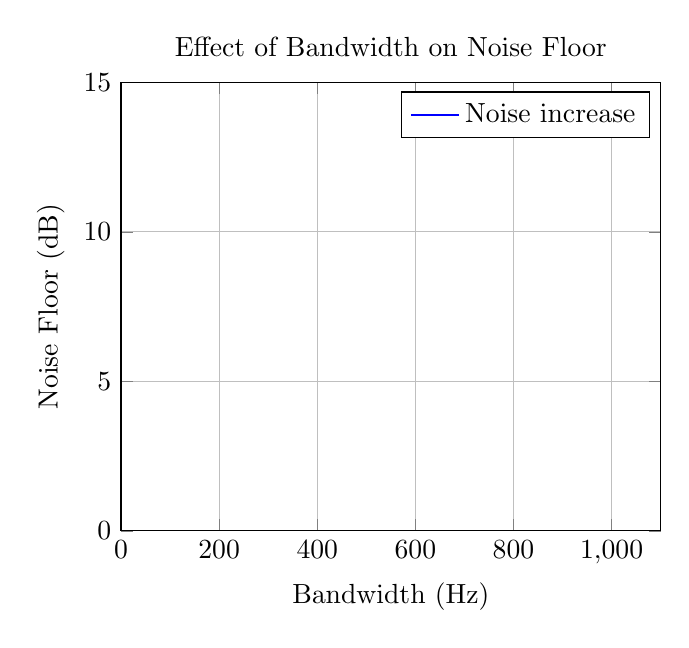
\begin{tikzpicture}
    \begin{axis}[
        xlabel={Bandwidth (Hz)},
        ylabel={Noise Floor (dB)},
        title={Effect of Bandwidth on Noise Floor},
        grid=both,
        ymajorgrids=true,
        xmajorgrids=true,
        xmin=0, xmax=1100,
        ymin=0, ymax=15,
        ticks=both,
        ]
        \addplot[color=blue, thick] {10*log10(x/50)};
        \addlegendentry{Noise increase}
    \end{axis}
\end{tikzpicture}
\end{center}
